\section{Results}


\captionsetup{font=small}
\begin{figure}[t]
    \centering
    \begin{minipage}[b]{0.2385\textwidth}
        \centering
        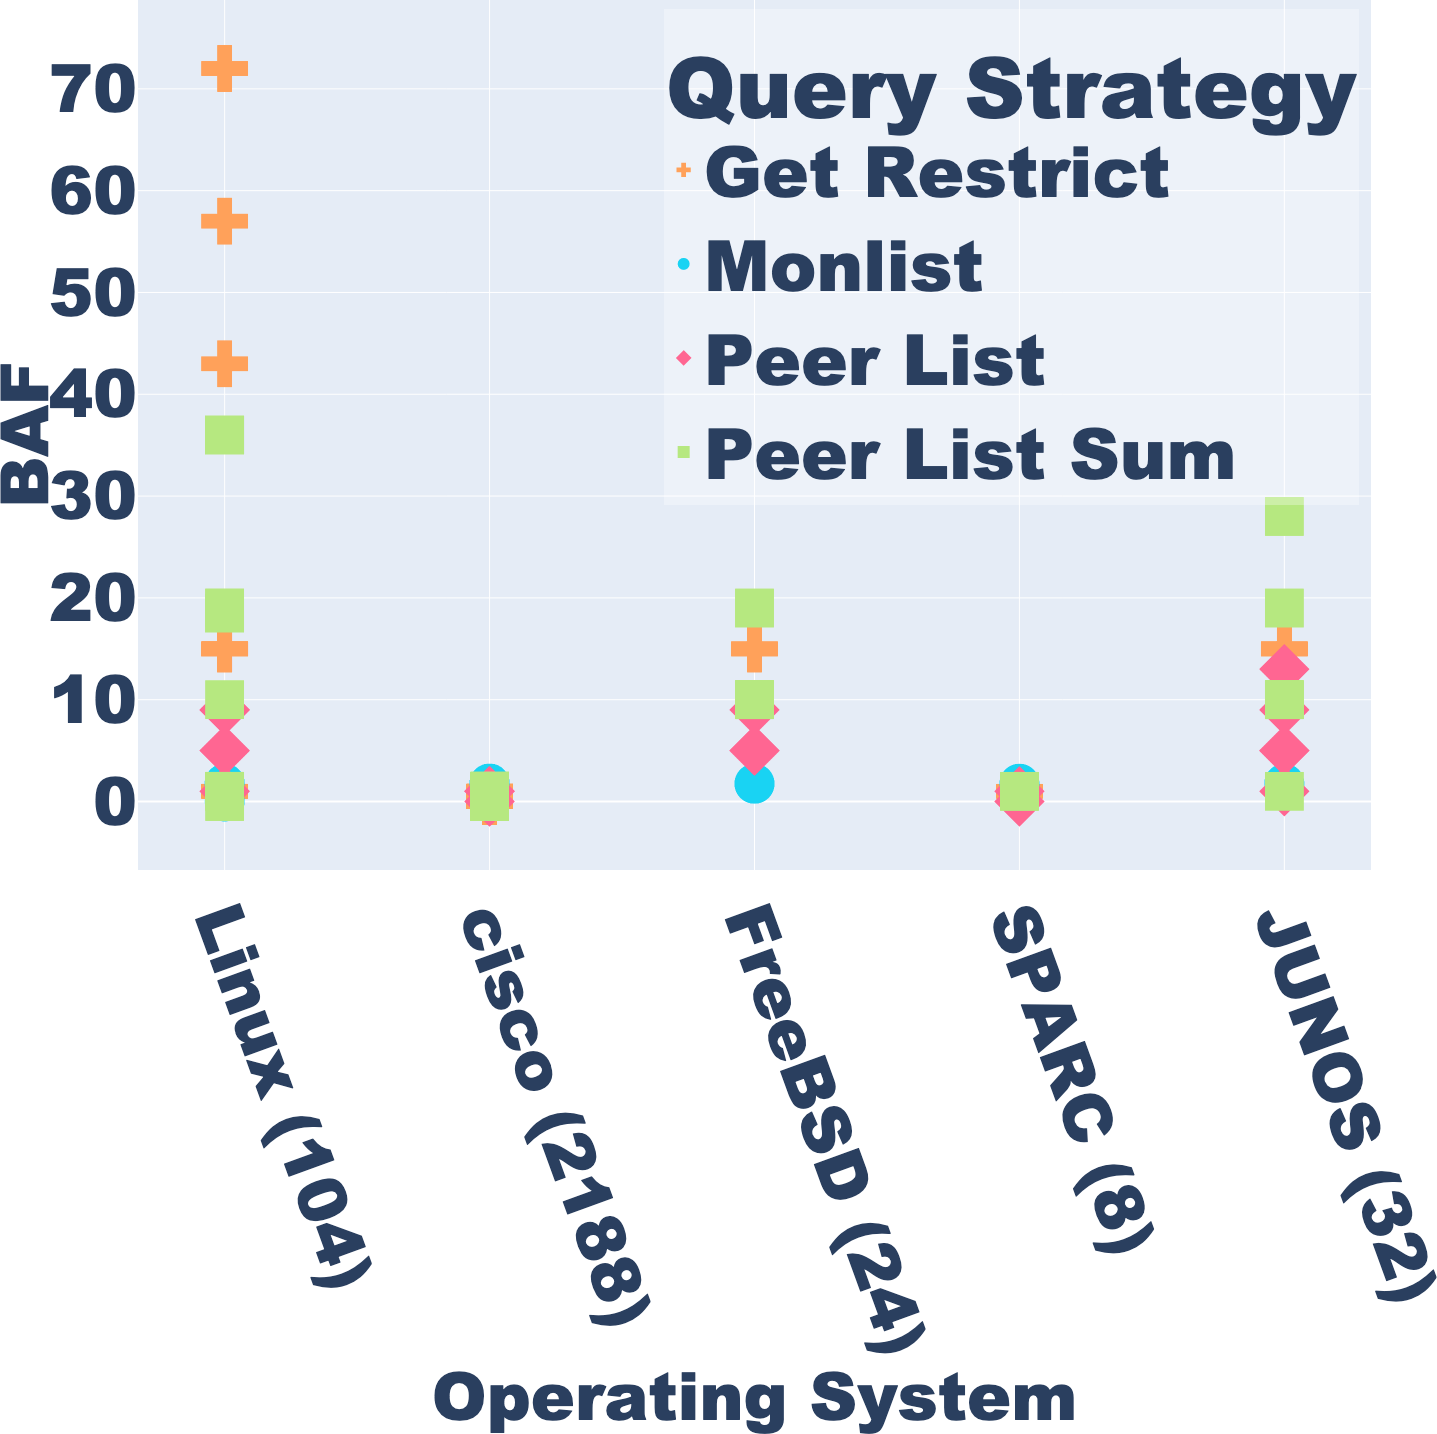
\includegraphics[width=\textwidth]{research paper/plots/ntp_systems_processed_all_trim.png}
        \caption{BAF (\# IPs) vs OS for NTP.}
        \label{fig:ntp_os}
    \end{minipage}
    \hfill
    \begin{minipage}[b]{0.2385\textwidth}
        \centering
        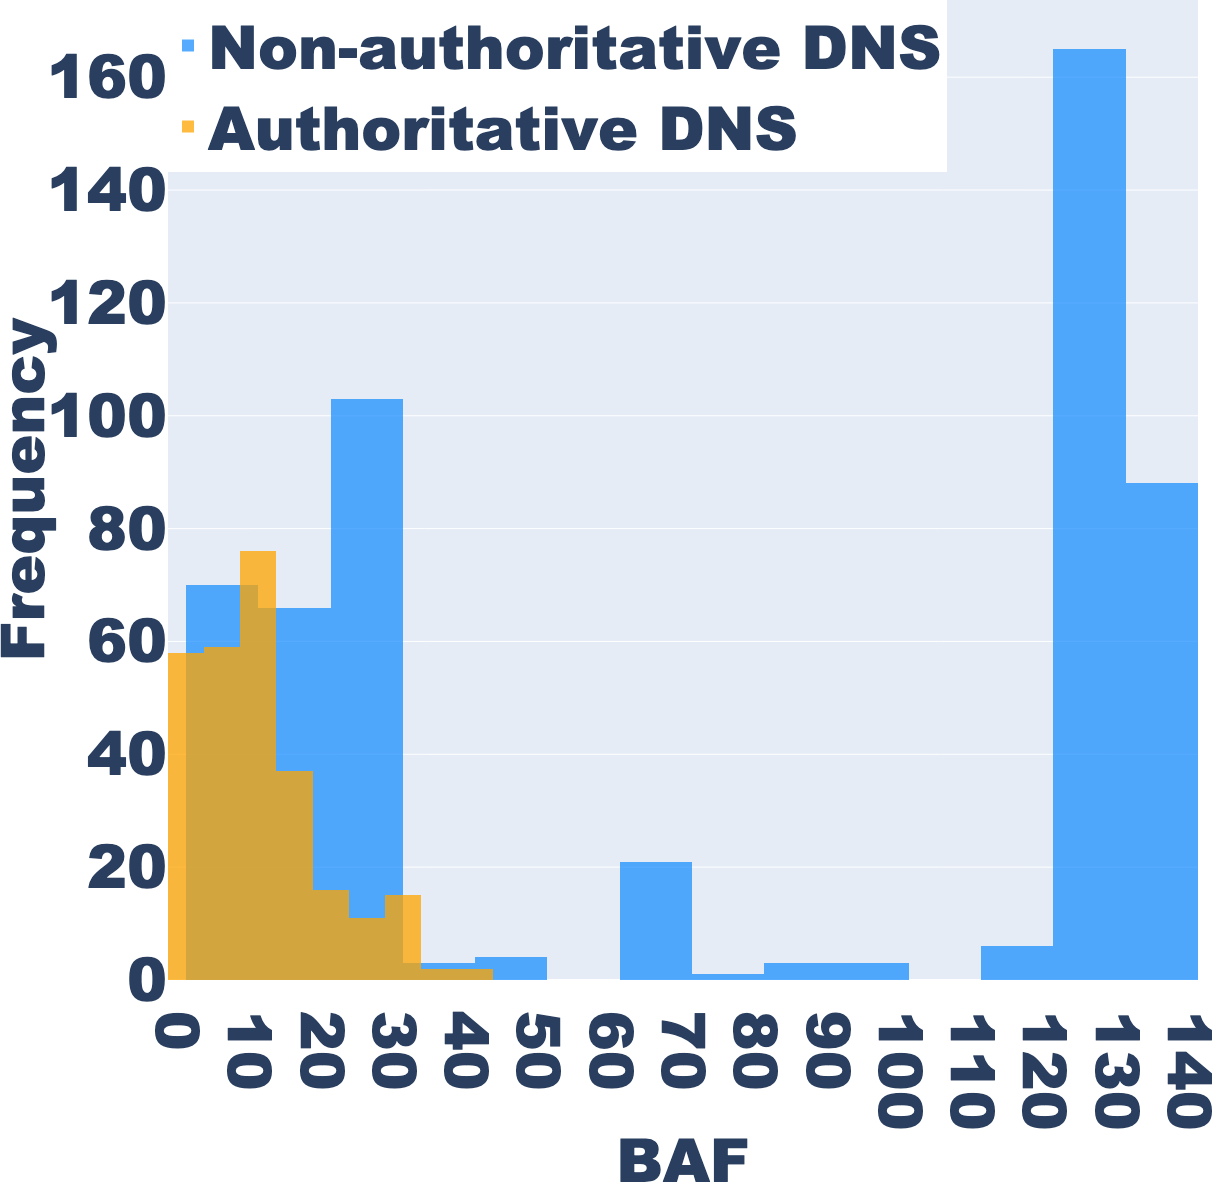
\includegraphics[width=\textwidth]{research paper/plots/dns_sl_histogram_incl_auth3_trim.png}
        \caption{DNS BAF comparison.}
        \label{fig:dns_auth_hist}
    \end{minipage}
\end{figure}


\looseness=-1 \textbf{Amplification attacks}. The amplification factors we achieved using the three protocols are shown in Table~\ref{tab:hosts_baf}. Note that for Memcached, none of the servers were open to UDP requests. Similarly, we did not find significant amplification factors for NTP, as observed previously~\cite{amplification_hell}. We attribute this to the effective campaign against private queries (specifically ``monlist'') done by~\cite{exit_hell}. Note that versions before 4.2.7p26 were vulnerable to traffic amplification via the ``monlist'' request~\cite{ntp_cve}. Still, as Fig.~\ref{fig:ntp_os} shows, some servers still respond to Mode 7 queries, which should not be the standard. Many hosts running Cisco OS have an amplification factor of 0, indicating they are well-configured. In contrast, Linux machines obtain the highest BAFs observed, likely due to misconfiguration. A detailed breakdown of the distribution of BAFs for NTP can be seen in Fig.~\ref{fig:piechart_ntp} in Appendix~\ref{appendix:piecharts_boxplots}. We have no quantitative results for Memcached as none of the servers responded to UDP, but a thorough discussion about what BAF could theoretically be achieved is presented in Appendix~\ref{appendix:measurement_queries}.


\looseness=-1 The story, however, is much different for DNS. This protocol can be weaponised to a large extent in the context of amplification attacks. The worst $250$ DNS amplifiers located in Greece cumulatively achieve an amplification factor of $32,087$. A histogram of the amplification factor of DNS servers is presented in Fig.~\ref{fig:dns_auth_hist}, which also shows that authoritative nameservers are more difficult to weaponize. Approximately 11\% of all open DNS servers achieved a BAF greater than 100. This should prove that such effective amplifiers would be relatively easy for an attacker to find in the wild. We further examined the relationship between the amplification factor and potential causes. The distribution of amplification factors can be seen in Fig.~\ref{fig:piechart_dns} in Appendix~\ref{appendix:piecharts_boxplots}.

\captionsetup{font=small}
\begin{figure}[t]
    \centering
    \begin{minipage}[b]{0.2385\textwidth}
        \centering
        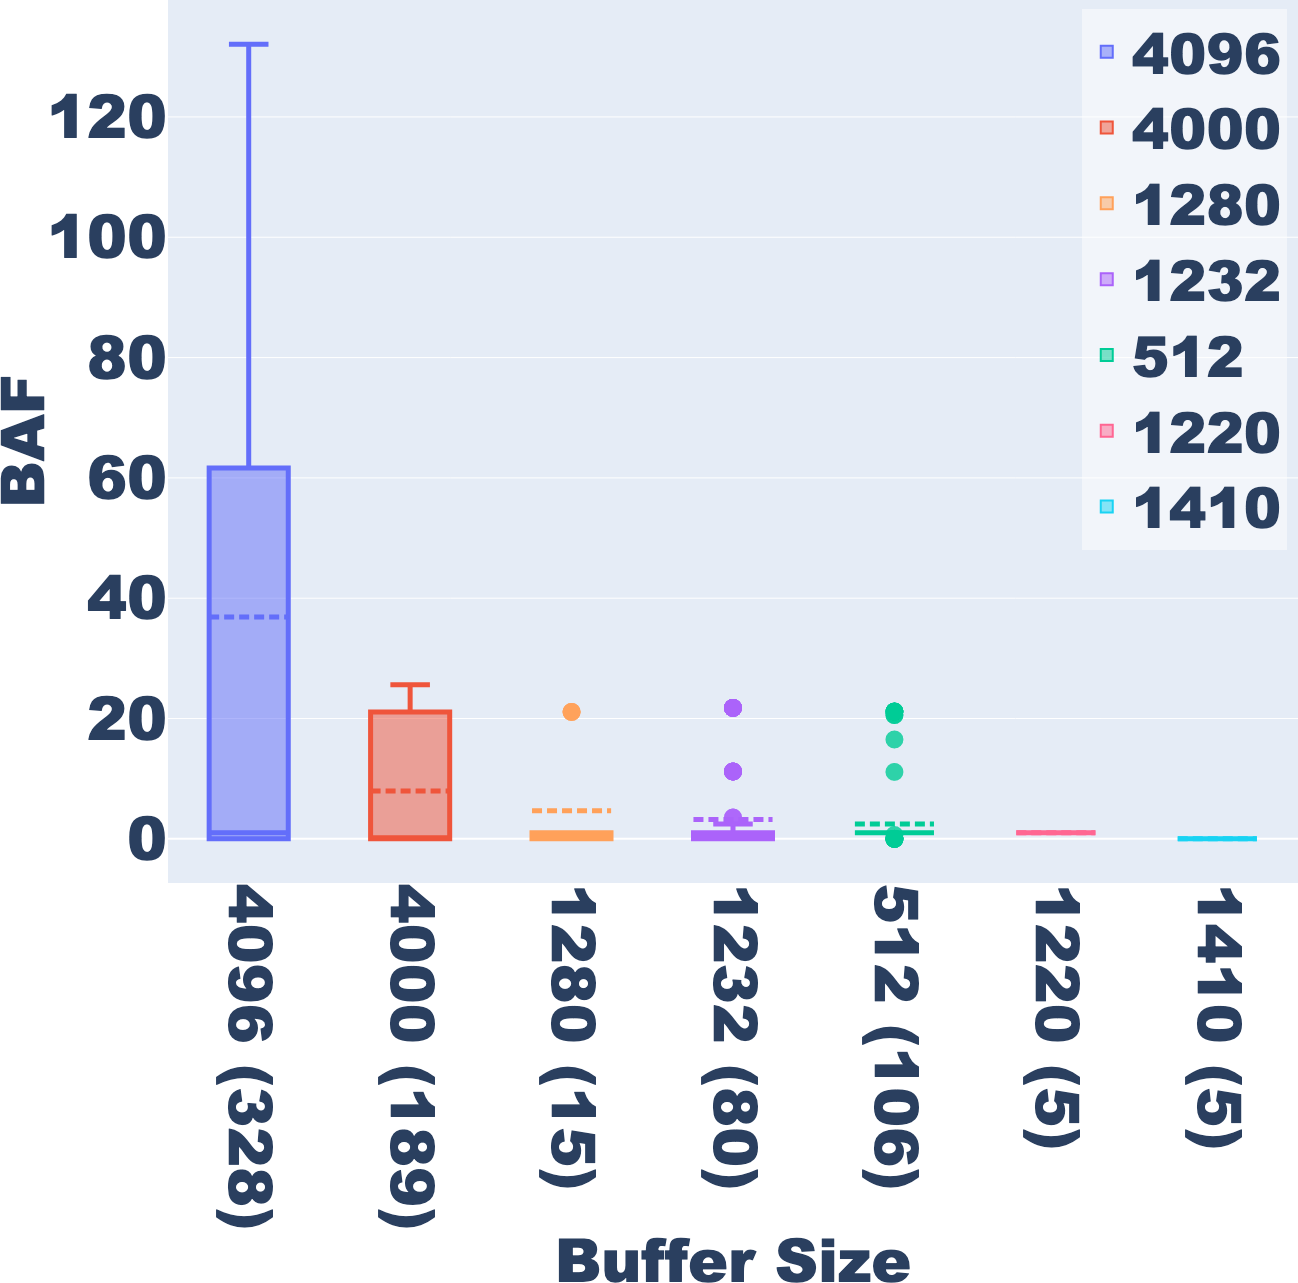
\includegraphics[width=1\textwidth]{research paper/plots/SL_boxplot_all_trim.png}
        \caption{BAF against Buffer Size (\# IPs).}
        \label{fig:boxplot_buffersize}
    \end{minipage}
    \hfill
    \begin{minipage}[b]{0.2385\textwidth}
        \centering
        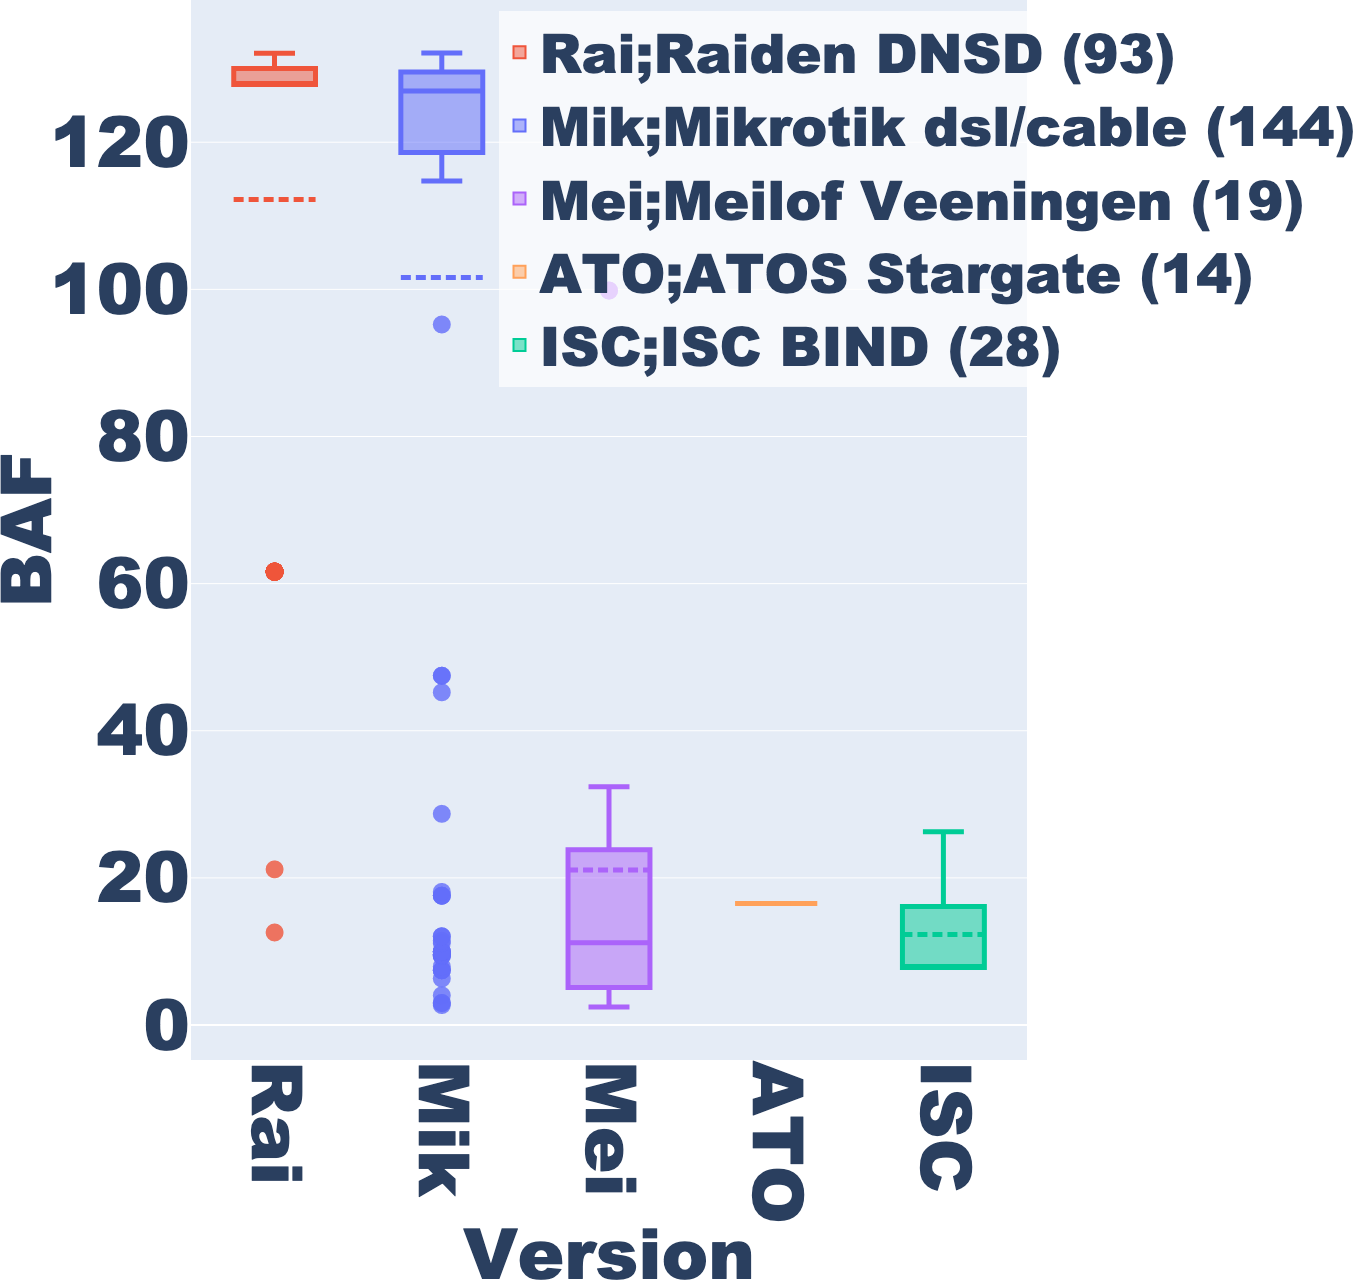
\includegraphics[width=1\textwidth]{research paper/plots/SL_boxplot_restricted_trim.png}
        \caption{BAF against DNS Version. The \# of IPs per group is shown in the legend.}
        \label{fig:fingerprint_boxplot}
    \end{minipage}
\end{figure}


\looseness=-1 \noindent \textbf{1. EDNS0 buffer size}. The introduction of the EDNS0 extension made DNS responses larger than $512$ bytes possible~\cite{rfc6891}. Clients can specify the maximum response size they can handle (rclass in the header), and similarly, hosts can optionally advertise the largest response size they accept \cite{edns0-primer}. After collecting the buffer size of our DNS hosts, we wanted to see if there was a positive correlation with the amplification factors, i.e., hosts that advertise a larger buffer size also attain a larger BAF. 

\looseness=-1 We observed that the hosts (whose buffer size we knew) that achieved the most significant amplification factors published a buffer size of $4,096$ (Fig.~\ref{fig:boxplot_buffersize}), where the median is situated around the value of 40. The CDF in Fig.~\ref{fig:cdf_buffer_size} also shows the noticeable amplification factors for the group that advertised a buffer size of $4,096$, $\approx 25\%$ of them achieve a BAF $\geq 100$ (around 82 hosts). The difference to the other groups is apparent, as the other 4 groups get a BAF of 20 at most. Note that we plotted the top 5 groups according to the mean BAF and only kept groups with at least 10 members. 

\looseness=-1 There have been attempts to discourage setting this considerable buffer size value since it can lead to IP Fragmentation~\cite{dnsflagday}. It has been strongly advised to set it to a value such as $1,232$, which should be enough for all practical purposes, as suggested by DNS flag day 2020~\cite{dnsflagday}, which was a collaborative initiative by DNS software and service providers to promote better DNS protocol compliance. Furthermore, a large buffer size significantly increases the amplification potential, making the problem two-fold. We have also observed cases where the buffer size is not correctly configured, i.e. a server advertises a value but does not truncate and switches to TCP when receiving a more extensive response. This happened, for instance, in the group that selected a buffer size of 512, then technically, the maximum attainable BAF should have been $\frac{512}{31} \approx 16.5$, but we can see in Fig. \ref{fig:boxplot_buffersize} that there is a small subset of hosts that achieved a BAF of $\approx 20$. 

\looseness=-1 We want to underline that $\approx$ $45\%$ of the hosts whose buffer size we know advertised a value of 4,096, and $\approx$ $70\%$ advertised a value $\geq 4,000$. These results are similar to the ones found by Van Rijswijk-Deij et al.~\cite{van_rijswijk-deij_dnssec_2014}, who found that the prevalent configuration (in 90\% of the servers that adopted EDNS0) for the buffer size was a value at least as high as 4,000 bytes. We obtained a slightly smaller result, likely due to a number of hosts adopting the DNS flag day recommendation; still, the vast majority advertised a large value for the buffer size (i.e. $\geq 4,000$).


\captionsetup{font=small}
\begin{figure}[t]
    \centering
    \begin{minipage}[b]{0.2385\textwidth}
        \centering
        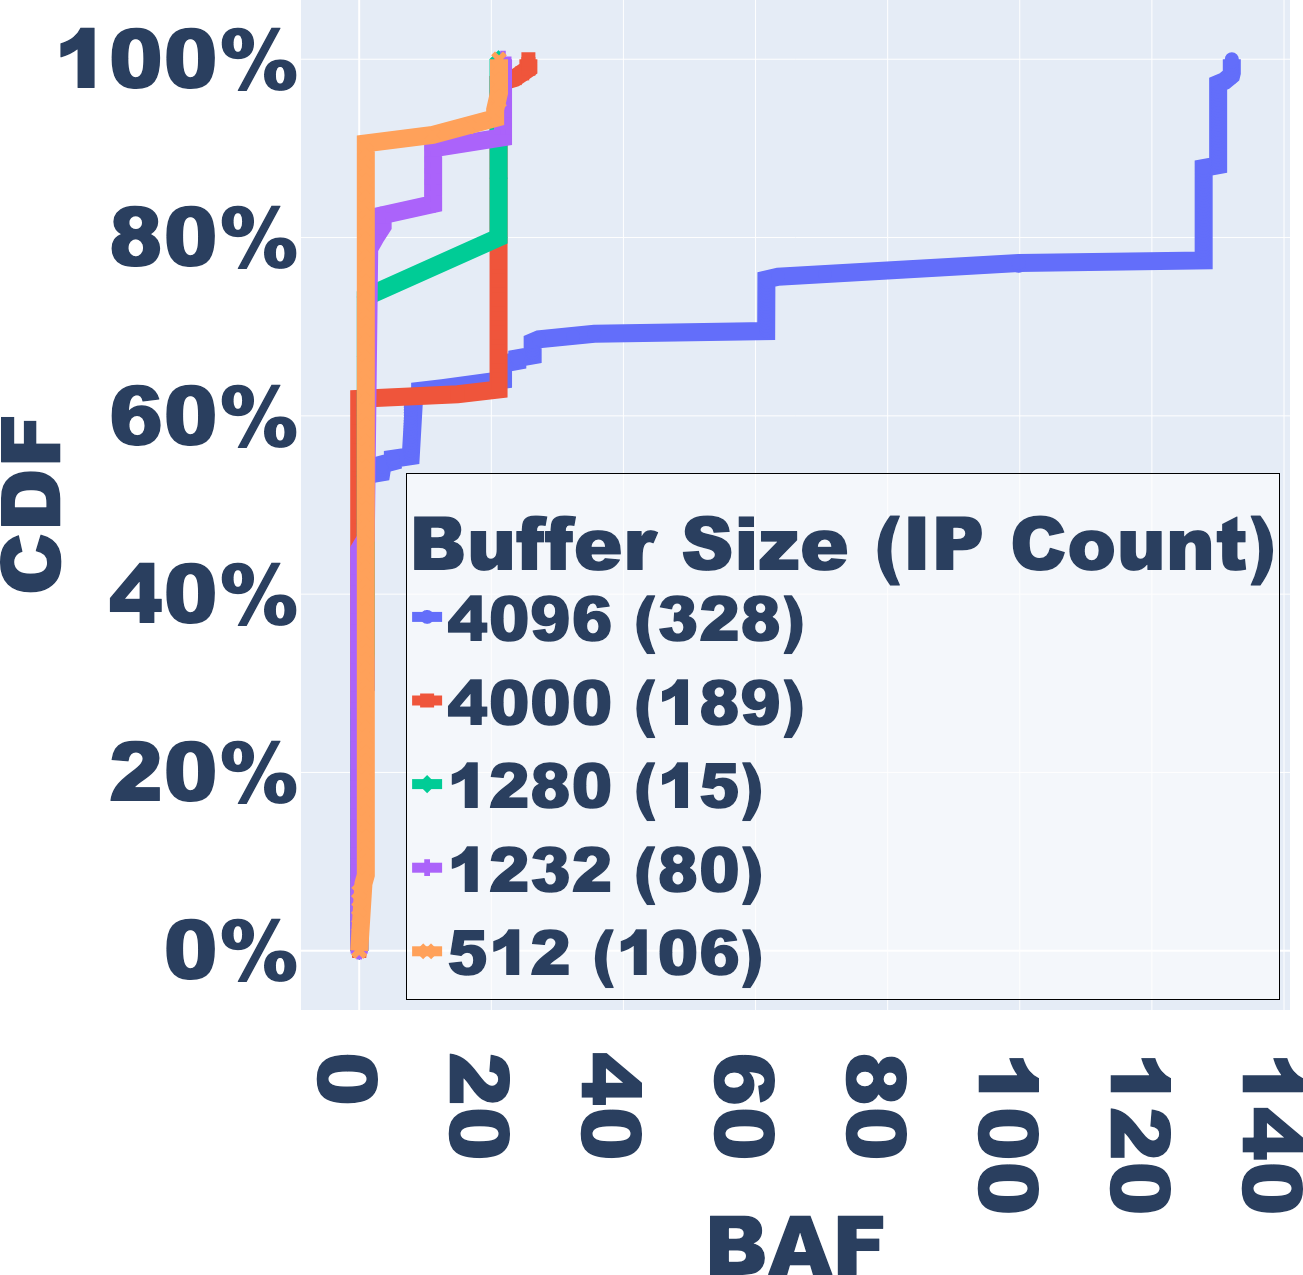
\includegraphics[width=\textwidth]{research paper/plots/SL_buffer_size_cdf_trim.png}
        \caption{CDF per Buffer Size.}
        \label{fig:cdf_buffer_size}
    \end{minipage}
    % \hfill
    \begin{minipage}[b]{0.2385\textwidth}
        \centering
        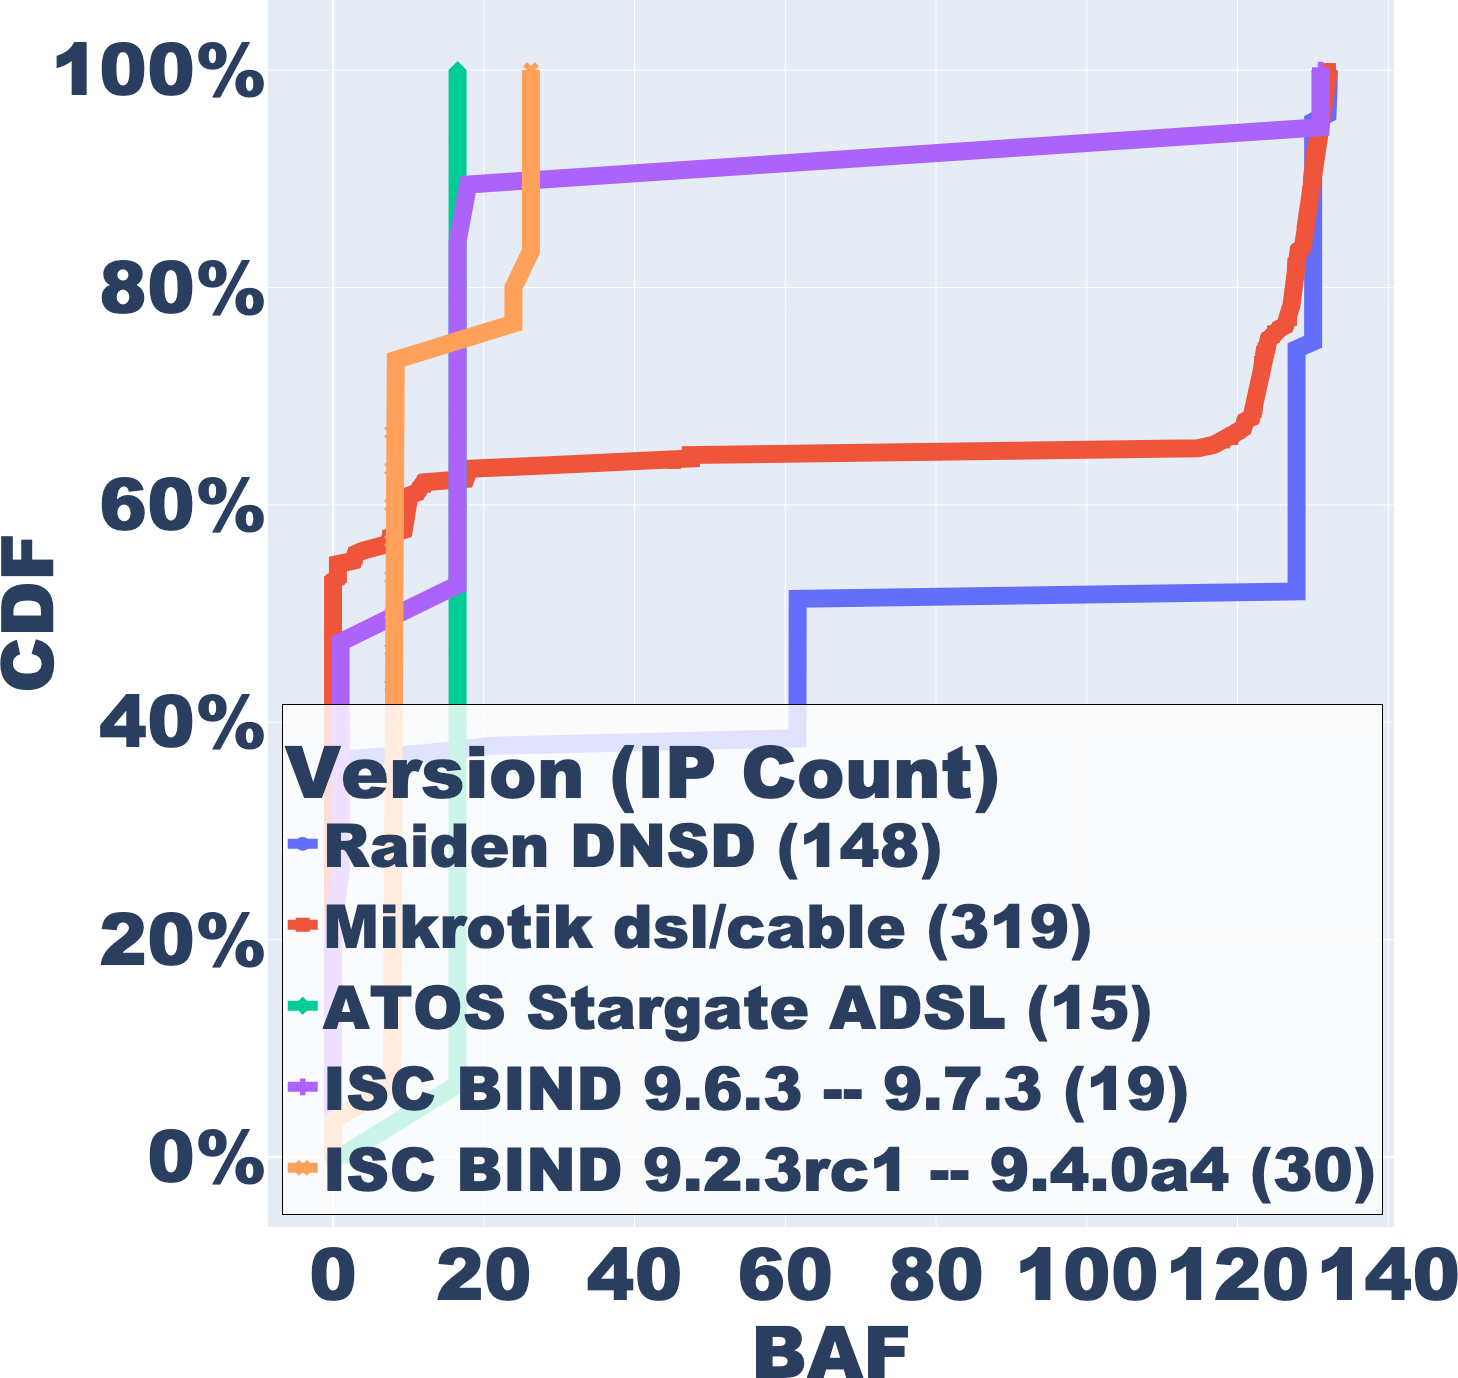
\includegraphics[width=\textwidth]{research paper/plots/SL_version_cdf_trim.png}
        \caption{CDF per Version.}
        \label{fig:cdf_version}
    \end{minipage}
\end{figure}

\looseness=-1 \noindent \textbf{2. DNS implementation}. We found two DNS versions (after running ``fpdns'') which achieved very high BAFs, namely Raiden DNSD and MikroTik. In Fig.~\ref{fig:fingerprint_boxplot}, we can see the mass of the two implementations centred around the substantial value of 120. Note that we have ignored hosts with BAFs $\leq$ 1 in this figure, as they are not considered amplifiers. With a closer inspection of the distribution of all hosts running the respective DNS software, we observe from the cumulative distribution function in Fig.~\ref{fig:cdf_version} that $\approx 50\%$ of all Raiden DNSD hosts have a BAF larger than 120. Similarly, the figure shows that $\approx 35\%$ of MikroTik hosts have a BAF $\geq$ 120. This amounts to around 74 Raiden and 111 MikroTik hosts with a BAF greater than 120. Since Fig.~\ref{fig:cdf_version} shows the top 5 groups according to the mean BAF (and whose group count is $\geq 10$), we see that there is a significant difference compared to the other 3 versions that are part of the top 5, ATOS Stargate and BIND 9.2.3rc1 - 9.4.0a4 can get at most a BAF of $\approx 20$. Only $\approx 10\%$ of hosts running BIND 9.6.3 - 9.7.3 obtain a BAF comparable to MikroTik and Raiden, i.e. $\geq 120$. However, this is still a tiny amount of servers compared to the other two (around 9). Furthermore, looking at the top 250 hosts according to the BAF obtained (regardless of whether we know their DNS implementation or not), we find that 175 of them are running either MikroTik or Raiden DNSD, that is 70\% of the top 250 hosts. The other 30\% (i.e. 75) of hosts are made up of 73 whose software we could not find, and the remaining two are running two different versions of BIND~\cite{bind}. 


\looseness=-1 We further investigate hosts that run one of these two DNS implementations to determine the root cause of their predisposition to high amplification. For Raiden, we have not been able to reach a meaningful conclusion using information from their website~\cite{raiden_dnsd}; however, plotting a heatmap of the buffer size advertised versus the DNS implementation in Fig.~\ref{fig:heatmap_buffer_version}, we notice that all of the Raiden servers that advertised a buffer size did so with a value of 4,096, which leads us to think that this is the preconfigured setting for the Raiden DNS implementation. 


\looseness=-1 For MikroTik hosts, we could not retrieve the buffer size empirically; thus, it is not present in the same heatmap. However, MikroTik DNS documents that the buffer size it uses by default is $4,096$~\cite{mikrotik_forum}. This leads us to assume that this default value and is likely not overridden by administrators. 

\captionsetup{font=small}
\begin{figure}[t]
    \centering
    \begin{minipage}[b]{0.2385\textwidth}
        \centering
        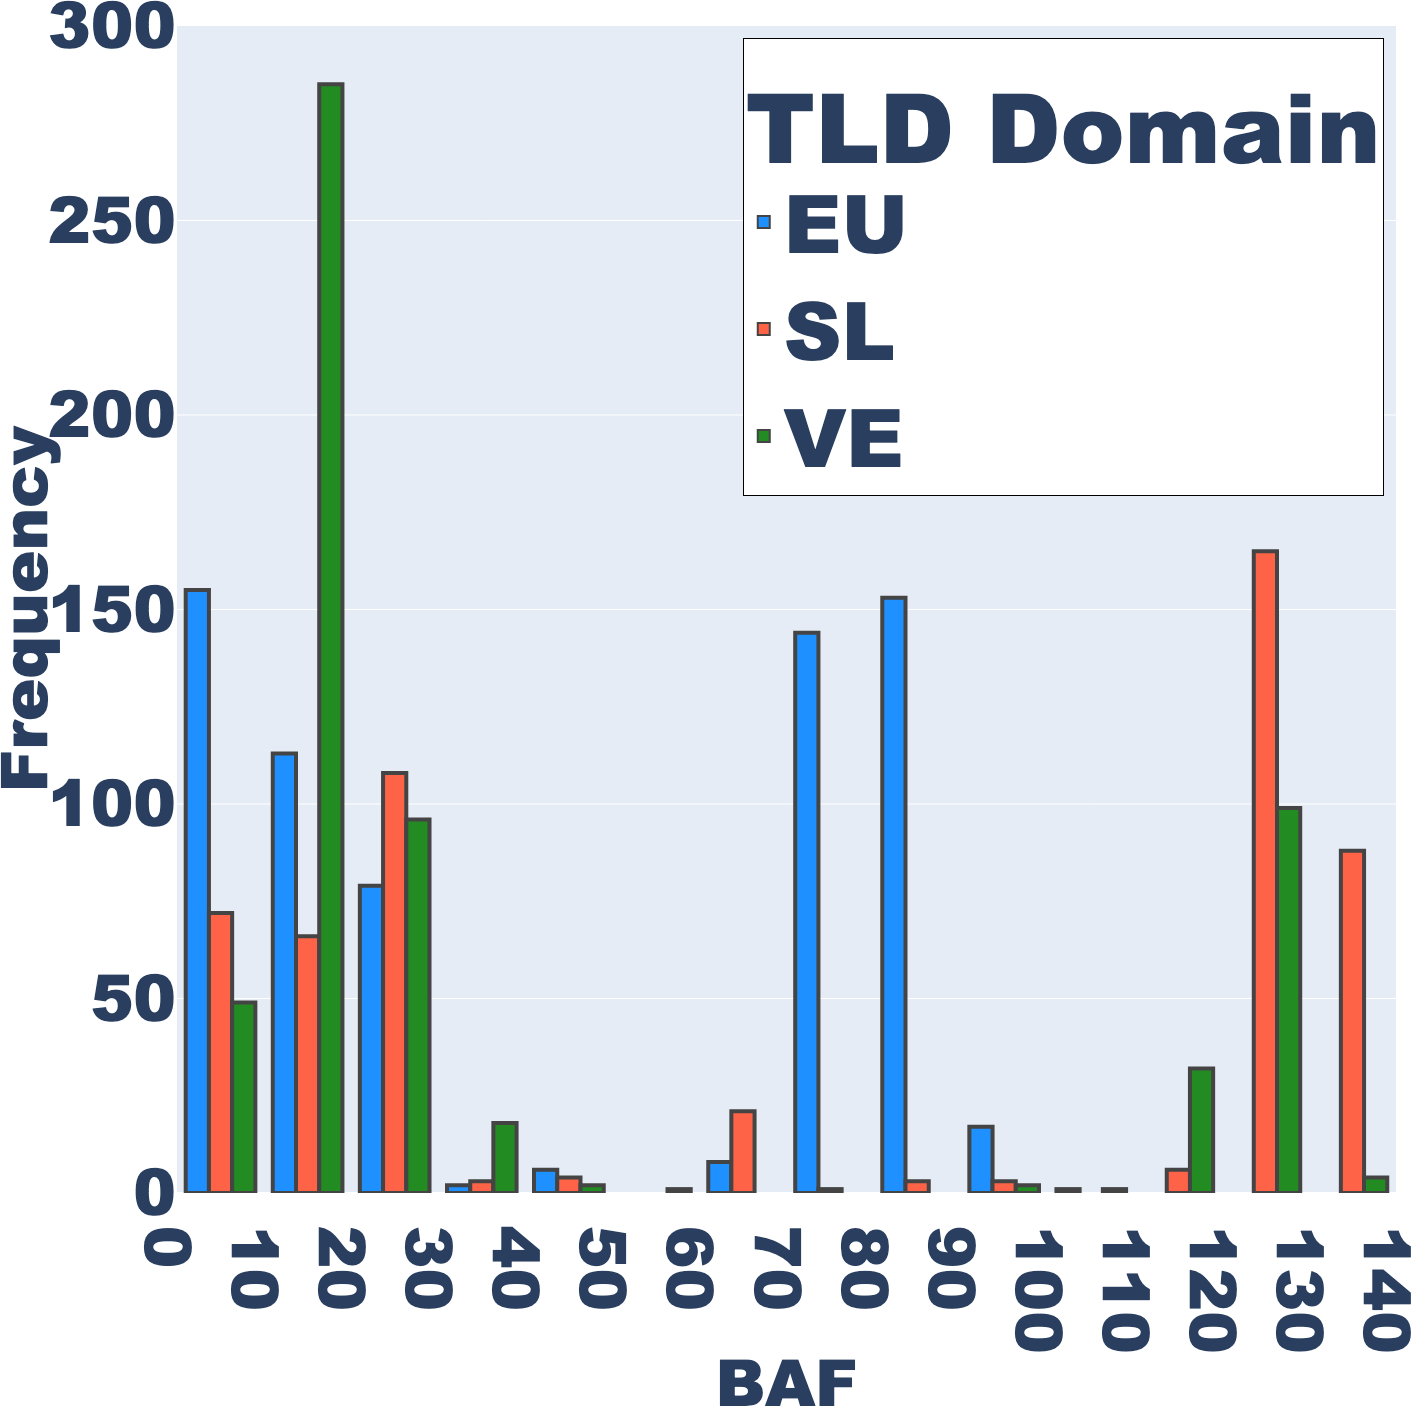
\includegraphics[width=\textwidth]{research paper/plots/dns_histogram_comparison_trim.png}
        \caption{BAFs for ``ANY'' on different domains.}
        \label{fig:any_diff_domains}
    \end{minipage}
    \hfill
    \begin{minipage}[b]{0.2385\textwidth}
        \centering
        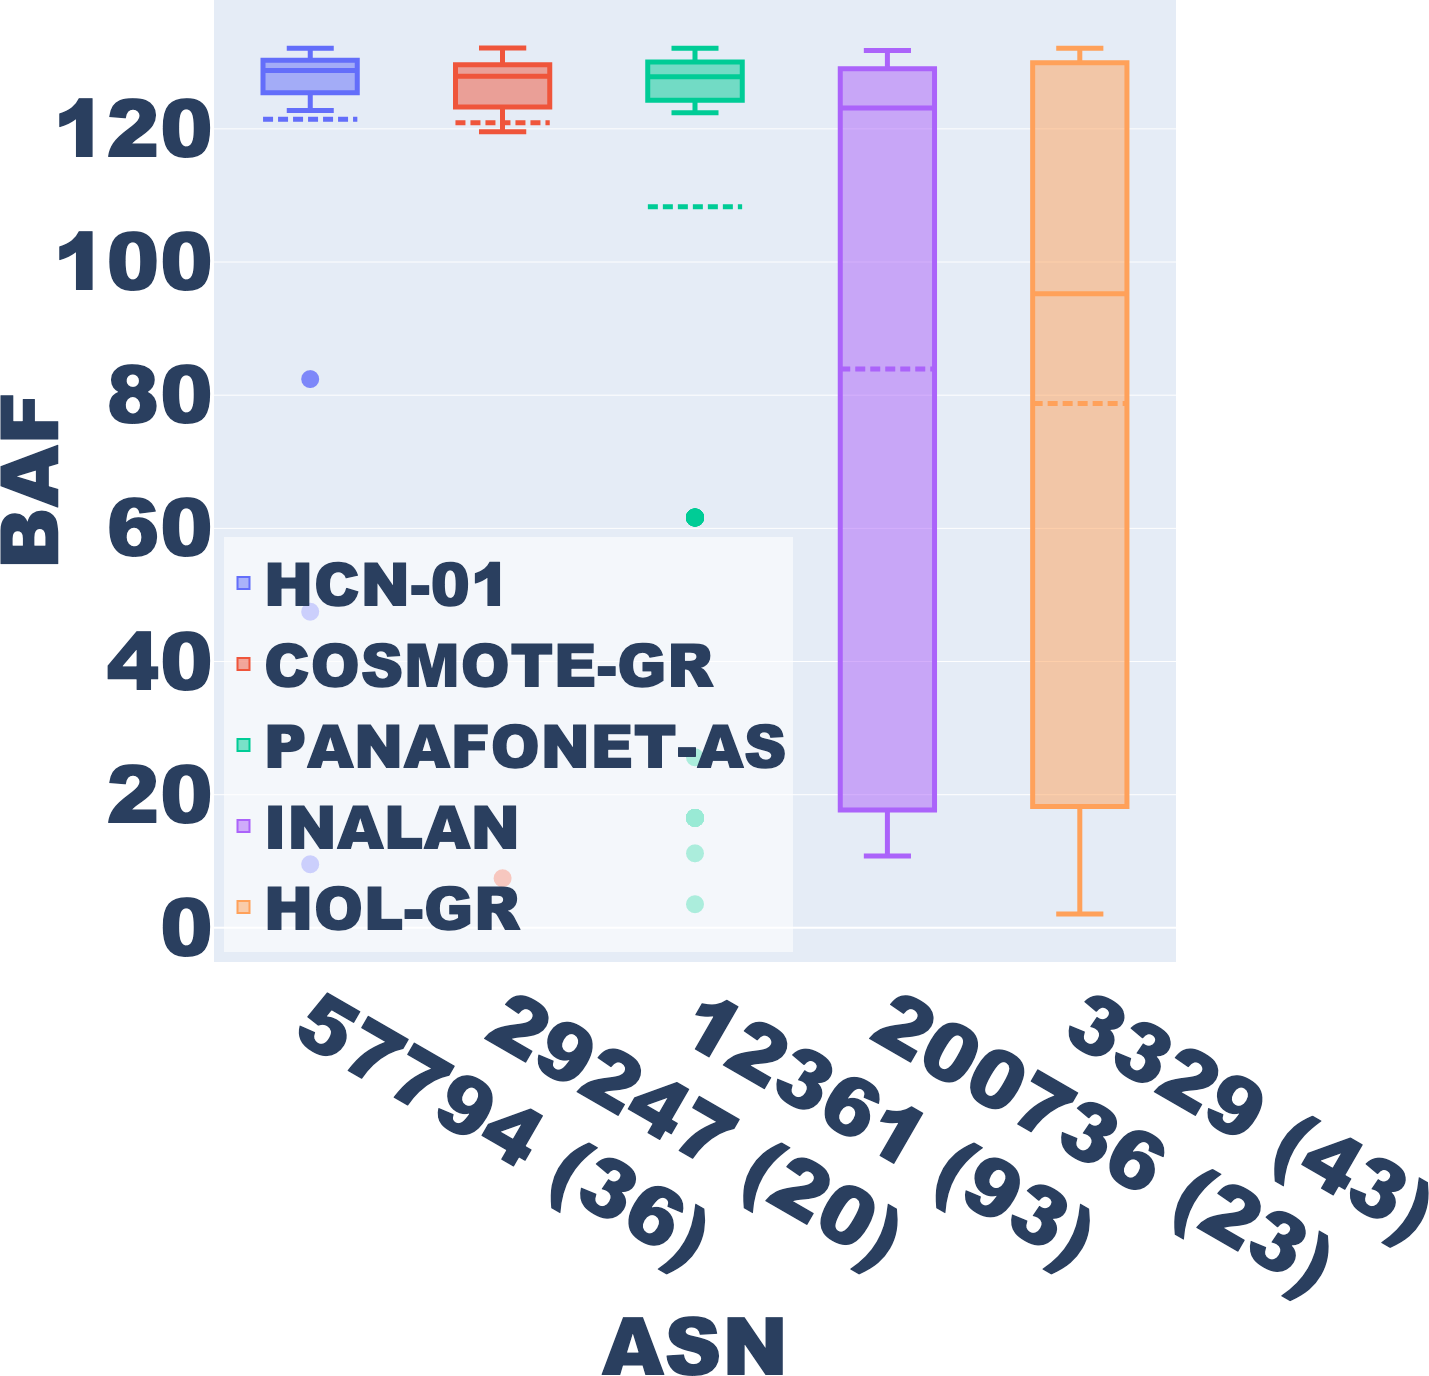
\includegraphics[width=\textwidth]{research paper/plots/SL_netw_boxplot_restricted_trim.png}
        \caption{BAFs per AS.}
        \label{fig:network_info}
    \end{minipage}
\end{figure}

\looseness=-1 \noindent \textbf{3. Domain}. Unsurprisingly, the domain queried plays a crucial role in the size of DNS responses. This is an area that an attacker might specifically optimise, i.e. choosing the best domain given a specific nameserver. Three TLDs (.eu, .sl and .ve) and the BAFs achieved are compared in Fig.~\ref{fig:any_diff_domains}. The figure shows that ``ANY'' gives the highest amplification for many hosts for the ``.sl'' TLD, whereas .ve also obtains high BAFs but with a much smaller frequency; we can see a peak in frequency for a BAF between 20 and 30. The ``.eu'' TLD obtains smaller BAFs, around 70 to 80, for a decent number of servers. Overall, .sl reliably gets very high BAF values (i.e., for numerous subsets of hosts). Note that many other domains might get comparable BAFs, and an attacker might try them all for each DNS server and only use the one that rewards them with the largest amplification factor. A complete measurement study of domains and their relationship to response size was done by Van Der Toorn et al.~\cite{van_der_toorn_anyway_2021}.

\begin{figure}[t]
    \centering
    \begin{minipage}[b]{0.2385\textwidth}
        \centering
        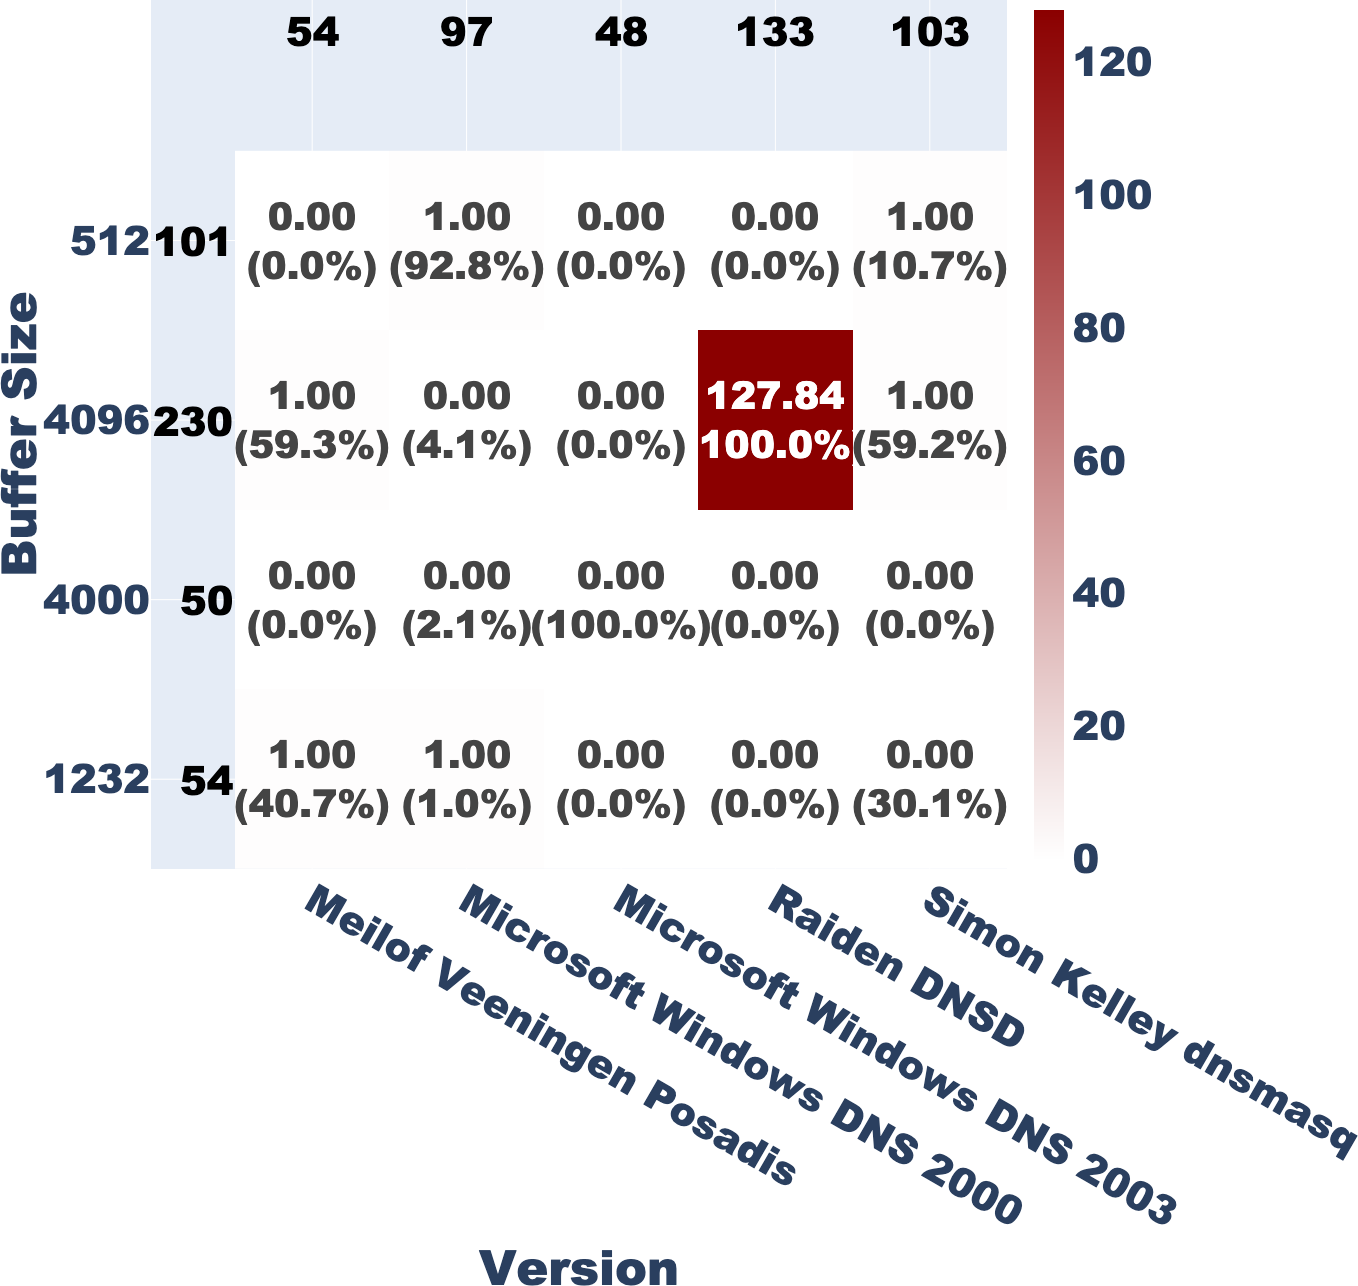
\includegraphics[width=\textwidth]{research paper/plots/filtered_Buffer Size_vs_Version_trim.png}
        \caption{Buffer Size against DNS software.}
        \label{fig:heatmap_buffer_version}
    \end{minipage}
    % \hfill
    \begin{minipage}[b]{0.2385\textwidth}
        \centering
        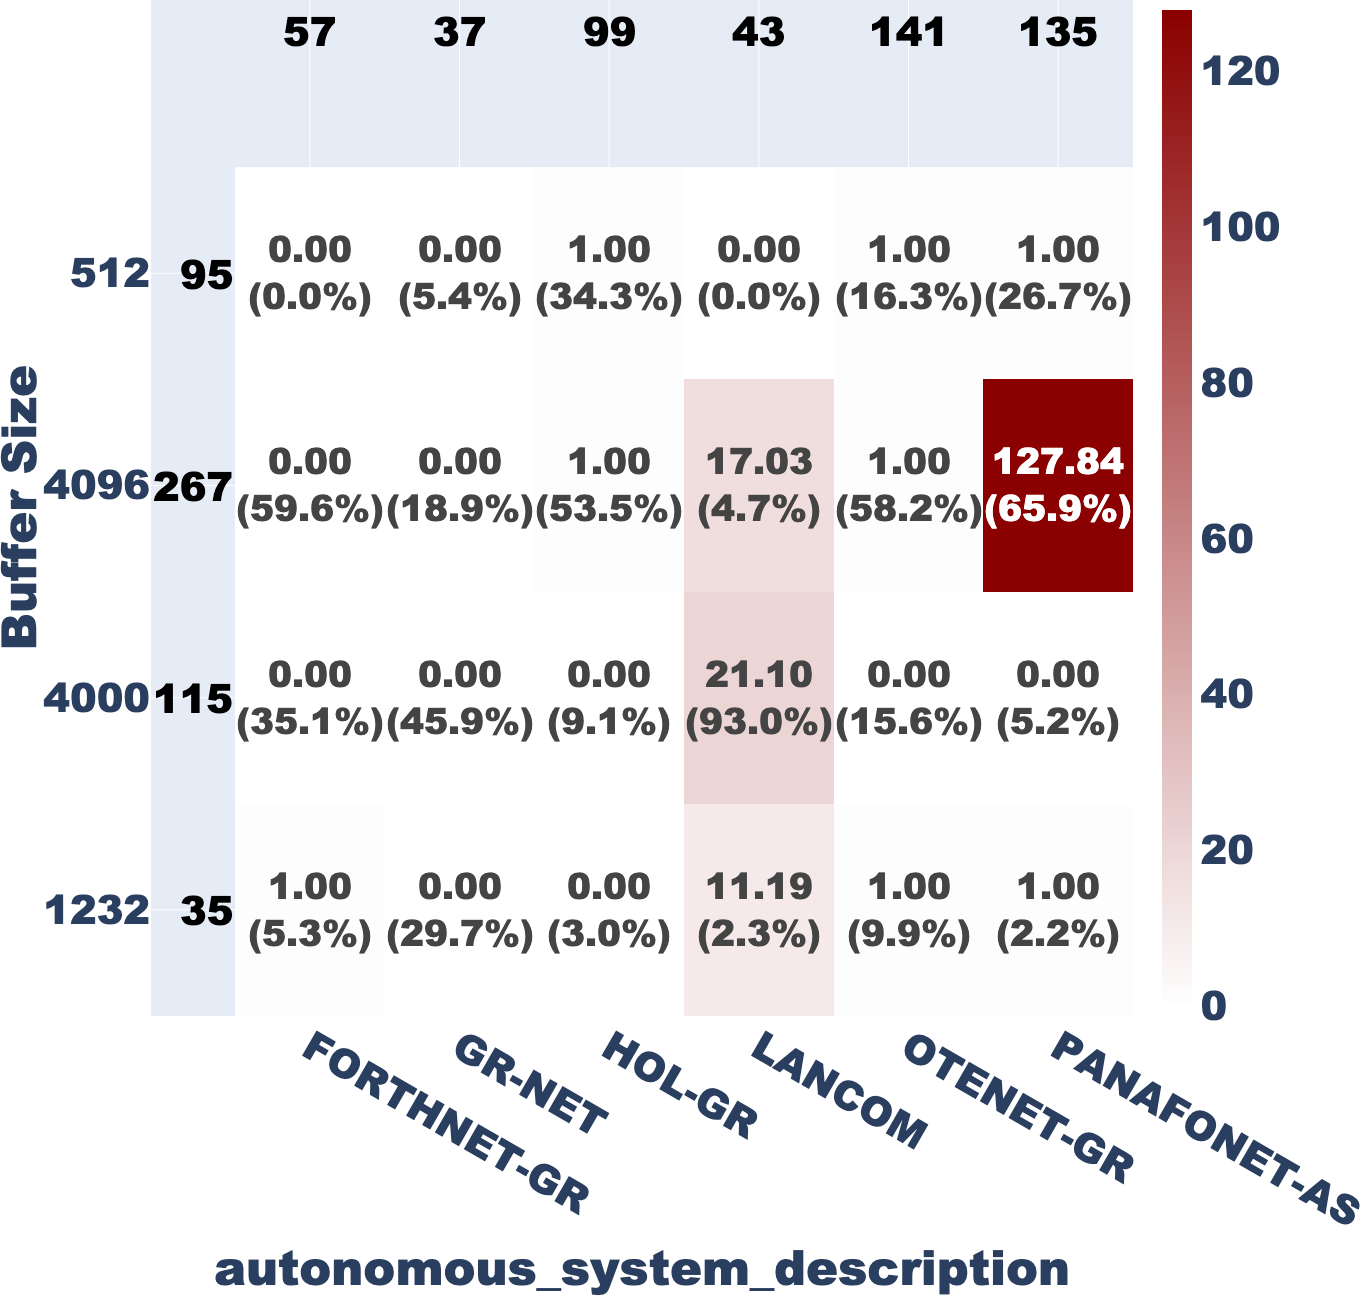
\includegraphics[width=\textwidth]{research paper/plots/filtered_Buffer Size_vs_autonomous_system_description_trim.png}
        \caption{Buffer Size against AS.}
        \label{fig:heatmap_buffer_as}
    \end{minipage}
\end{figure}

\looseness=-1 \noindent \textbf{4. AS}. Looking at the networks where hosts are situated, we noticed that some ASs are more vulnerable than others, as depicted in Fig.~\ref{fig:network_info}. Note that this does not imply something inherently wrong with these networks, but rather that there are vulnerable hosts with likely misconfigured settings (such as the EDNS0 buffer size), see in Fig.~\ref{fig:heatmap_buffer_as}. We note that the first 3 ASs have most of their mass concentrated around the value of 120. Additionally, out of the top 250 hosts, according to their BAF, 123 of them are in one of the three ASs. In Fig.~\ref{fig:heatmap_buffer_as}, we see a heatmap of the buffer size against the AS description, and we can observe that the third AS from Fig.~\ref{fig:network_info} achieves the highest median BAF of $127.84$, and 65.9\% of its hosts advertise a buffer size of 4,096. This heatmap should further prove that there is a clear tendency to obtain a higher BAF if a larger buffer size is advertised. 



\looseness=-1 \noindent \textbf{5. Product and Vendor}. We have noticed that 99\% of hosts running RouterOS (from the vendor MikroTik) use the MikroTik DNS software but achieve very small BAFs, as it can be seen in Fig.~\ref{fig:heatmap_version_product} in Appendix~\ref{appendix:heatmaps}, where the median BAF of this group is 0. Interestingly, two other groups run the same DNS software and tend to get a high median amplification factor, namely 121.94 and 120.92 for hosts running DSM (from the vendor Synology) \cite{dsm} and servers running Linux, respectively. This ties in with the information that MikroTik DNS servers may advertise a buffer size of $4,096$ by default. Hosts that run RouterOS and MikroTik DNS are not affected by the large default buffer size, likely due to other cautionary measures that might have been implemented, such as answering with a HINFO RR to ``ANY'' queries, as has been advised by RFC8482 to provide minimally sized responses to ``ANY''~\cite{rfc-8482}. More details about the BAFs achieved by different vendors and products are presented in Figs.~\ref{fig:boxplot_vendor} and ~\ref{fig:boxplot_product}.
     

\looseness=-1 \textbf{Looping Attacks}. Our hosts are vulnerable to loopy attacks, as we found a few loops among the same protocol server pairs. A summary is shown in Table~\ref{tab:loops}. Note that we have not analysed cross-protocol vulnerabilities. 

\captionsetup{font=normalsize}
\begin{table}[t]
    \centering
    \caption{DNS and NTP Loops.}
    \normalsize
    \renewcommand{\arraystretch}{0.7} % Adjust row height
    \setlength{\tabcolsep}{1pt} % Adjust column spacing
    \begin{tabularx}{\columnwidth}{XXXXX}
    \toprule
    Protocol & Cycle & $\#\ of$ Involved IPs & Min Edge IP Amount & $\#\ of$ Pairs \\
    
    \midrule
    DNS & {[49, 49]} & 3 & 3 & 3 \\
    DNS & {[3, 3]} & 3 & 3 & 3 \\
    NTP & {[2, 2]} & 2 & 2 & 1 \\
    \midrule
    \multicolumn{4}{c}{Number of all affected IPs (DNS): 5} \\
    \multicolumn{4}{c}{Number of all affected IPs (NTP): 2}  \\
    \bottomrule
    \end{tabularx}
    \label{tab:loops}
\end{table}

\vspace{-5pt}

